%%
%% Modified 2016 September
%%
%% This is a sample manuscript marked up using the
%% AASTeX v6.1 LaTeX 2e macros.
%%
%% AASTeX is now based on Alexey Vikhlinin's emulateapj.cls 
%% (Copyright 2000-2015).  See the classfile for details.
%%
%% using aastex version 6.1
\documentclass[twocolumn]{aastex61}
\newcommand{\vdag}{(v)^\dagger}
\newcommand\aastex{AAS\TeX}
\newcommand\latex{La\TeX}
\usepackage{CJKutf8}
\usepackage{graphicx} 
\usepackage{subcaption} 
\usepackage{caption} 


%% Reintroduced the \received and \accepted commands from AASTeX v5.2
%\received{July 1, 2016}
%\revised{\today}
%\accepted{\today}
%% Command to document which AAS Journal the manuscript was submitted to.
%% Adds "Submitted to " the argument.
%\submitjournal{ApJ}


%% If you wish, you may supply running head information, although
%% this information may be modified by the editorial offices.
\shorttitle{\aastex\ Supernovae Across Ten Billion Years}
\shortauthors{Brown et al.}
%%
%% You can add a light gray and diagonal water-mark to the first page 
%% with this command:
%\watermark{DRAFT \today}
%% where "text", e.g. DRAFT, is the text to appear.  If the text is 
%% long you can control the water-mark size with:
%  \setwatermarkfontsize{dimension}
%% where dimension is any recognized LaTeX dimension, e.g. pt, in, etc.
%%
%%%%%%%%%%%%%%%%%%%%%%%%%%%%%%%%%%%%%%%%%%%%%%%%%%%%%%%%%%%%%%%%%%%%%%%%%%%%%%%%

%% This is the end of the preamble.  Indicate the beginning of the
%% manuscript itself with \begin{document}.

\begin{document}

\title{Galaxy Contamination in Galactic Reddening Maps}

%%  http://www.astro.ucla.edu/~wright/CosmoCalc.html
%%  z=4 --> 12.2 Gyr light travel time, age of universe 1.6 Gyr
%%  z=2 --> 10.4 Gyr light travel time, age of universe 3.3 Gyr
%%


%% Please use multiple 
%% \affiliation calls for to document more than one affiliation.
%%

\correspondingauthor{Peter J. Brown}
\email{pbrown@physics.tamu.edu}

\author[0000-0001-6272-5507]{Peter J. Brown}
\affil{Department of Physics and Astronomy,
Texas A\&M University, 4242 TAMU, College Station, TX 77843, USA }
\affil{George P. and Cynthia Woods Mitchell Institute for Fundamental Physics \& Astronomy}


\author{Tate Walker}
\affil{Department of Aerospace Engineering,
Texas A\&M University, 4242 TAMU, College Station, TX 77843, USA }

%%%%%%%%%%%%%%%%%%%%%%%%%%%%%%%%%%%%%%%%%%%%%%%%%%%%%%%%%%%%%%%%%%%%%%%%%%%%%%%%%

%% Mark off the abstract in the ``abstract'' environment. 
\begin{abstract}


\end{abstract}

%%%%%%%%%%%%%%%%%%%%%%%%%
\keywords{dust: general, Milky Way: dust, doing things right}


%%%%%%%%%%%%%%%%%%%%%%%%%%%%%%%%%%%%%%%%%
\section{Introduction} \label{sec:intro}

As luminosity is a fundamental property of astrophysical objects, properly correcting for the attenuation of light due to dust extinction is important.  Accurate luminosities are needed for calculating energy budgets, sizes of objects, and the calibration and use of astrophysical objects as standard candles to measure distances in the universe.

Dust extinction can occur anywhere along the line of sight from an object to the observer where there could be dust, including circumstellar dust, dust in the host galaxy of an object, circumgalactic dust, intergalactic dust, and dust in our own Milky Way galaxy.  These multiple components can make it complicated, but it is usually assumed that the component of dust extinction arising from the MW is the best understood.  The all-sky dust reddening maps of \citet{Schlegel_etal_1998}, hereafter referred to as SFD98, calibrated the luminosity at 100 $\mu$m from COBE/DIRBE and IRAS/ISSA to dust reddening using the colors of elliptical galaxies.  These maps have made it convenient to look up the SFD98 reddening (or the rescaling by \citealp{Schlafly_Finkbeiner_2011}) via the NASA Extragalactic Database (NED\footnote{\url{https://ned.ipac.caltech.edu/}}; \citealp{Mazzarella_etal_2001}) or other electronic queries without having to understand the data or read the paper or even the warnings from NED\footnote{\url{https://ned.ipac.caltech.edu/classic/help/faq3.html\#3a}}.  Combined with the mean value of R$_V$=3.1 from \citet{Fitzpatrick_1999} and ignoring the variations in the Milky Way \citep{Clayton_Cardelli_1988} one has the extinction as a function of wavelength or can also implicitly assume those as well as the elliptical galaxy spectrum used by SFD98 and have the extinction readily computed in a number of common passbands.

{\bf note: Given the warning of \citealp{Cardelli_etal_1989} that "Even lines of sight with R$_V$ $\simeq$ 3.1 deviate asmuch from these standard extinction laws as from the CCM
expression, and the deviations become increasingly large and
systematic as R$_V$ deviates from 3.1" makes one wonder why we feel we can correct for extinction at all.  }

\citet{Dalcanton_etal_2009} mentioned in a footnote that the SFD98 maps were contaminated by M82, brought to our knowledge through studies of the extinction toward the supernova (SN) 2014J \citep{Foley_etal_2014J}.  \citet{Johnson_etal_2009} cautioned about not just the contamination of M81 and M82 but also the highly variable region nearby.  As dust reddening from anywhere has strong consequences in the ultraviolet, the authors were led to ask the question ``What other galaxies might be contaminated in this same way?''

In this short paper we describe how we searched for examples of contaminating galaxies and give a table of recommended extinction values for the ones we found.  


%%%%%%%%%%%%%%%%%%%%%%%%%%%%%%%%%%%%%%%%%%
\section{Analysis} \label{sec_analysis}
  

Having one example to work from, the nearby, extreme starburst galaxy M82, we began our search by looking at the next eleven closest galaxies hosting supernovae observed by Swift (see e.g. \citealp{Brown_etal_2015_10}).  

compare with near-infrared K-band brightness




To detect higher A$_V$ sources in the dust maps, we decided to look up the value of A$_V$ at the center of each galaxy and 20\arcmin away in each of the four cardinal directions.  We could then individually examine sources which were significantly higher than the mean of the 20\arcmin radius.  As a baseline for what a significant excess is, we first looked up those values for 102 random positions in the sky.  
We looked up the values for each of the extragalactic sources in \citet{Rice_etal_1998}, the 70 brightest of which should already have been removed from the SFD98 maps.  For our scientific purposes, we also examined the nearby host galaxies used to calibrate the Cepheid-Supernova Ia distance ladder \citep{Riess_etal_2016}, over 700 supernova host galaxies observed by Swift \citep{Brown_etal_2014_SOUSA}.  
The central and mean radial values are plotted in Figure \ref{fig_av}.  

Most of the data cluster around the 1:1 line.  From the random positions, we set one and two sigma limits of 12 \% and 22\% which encompass 68\% and 95\% of the points, respectively.  We manually examine all points for which the central position has an A$_V$ of 12\% greater than (or less than) the mean of the points at 20 \arcmin.  


Some sources appear to be partially removed, replacing the pixels with the median value of a nearby annulus.   


Other values are not properly corrected for.
In the case of M31

The recommended value for the region around M31, as given in Appendix C of \citet{Schlegel_etal_1998},  is E(B-V)=0.062.  This is the value obtained from the NASA Extragalactic Database\footnote{https://ned.ipac.caltech.edu/} when searching the position of M31.  Since M31 is not removed from the maps, however, one obtains a value of E(B-V)=0.69 from the NASA/IPAC Infrared Science Archive from the website\footnote{https://irsa.ipac.caltech.edu/frontpage/} or python's astroquery.


\begin{figure*}
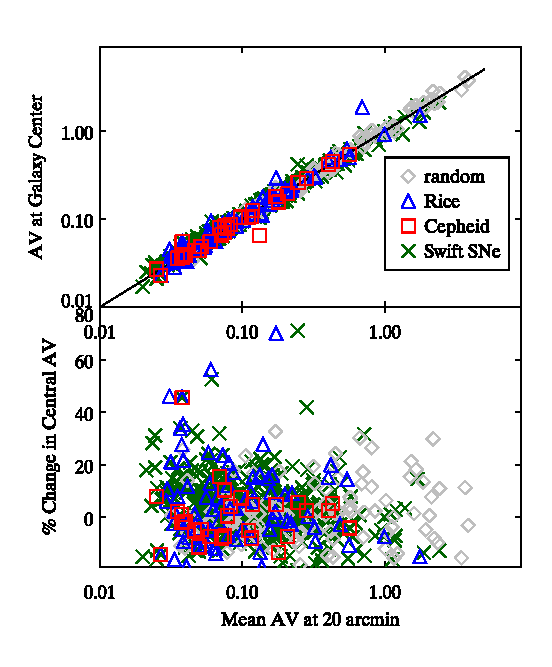
\includegraphics{avboth.eps}
\caption{Top panel: The central value of A$_V$ is plotted with respect to the mean of the A$_V$ values 20\arcmin away in each of the four cardinal directions.  102 random positions are plotted in grey.  The sample from \citet{Rice_etal_1998} which should have already been removed are blue triangles.  Nearby galaxies used to calibrate the Cepheid-SN distance ladder \citep{Riess_etal_2016} are plotted as red triangles.  The sample of Swift supernovae are green triangles.  A 1:1 line shows perfect agreement between the values.
Bottom panel: A$_V$ differences normalized by the mean A$_V$ at 20\arcmin.  The fractional difference is fairly constant with A$_V$.  
The fractional differences for the random locations have a standard deviation of 12\%.  This is used as the cutoff for 
\label{fig_av}}
\end{figure*}



\begin{figure}
\includegraphics{av_both.eps)
\caption{Left Panel: galaxies  Right Panel: A$_V$ v. radius from center in the four cardinal directions.
\label{fig_av}}
\end{figure}



\begin{figure}
  \begin{subfigure}[b]{0.4\textwidth}
    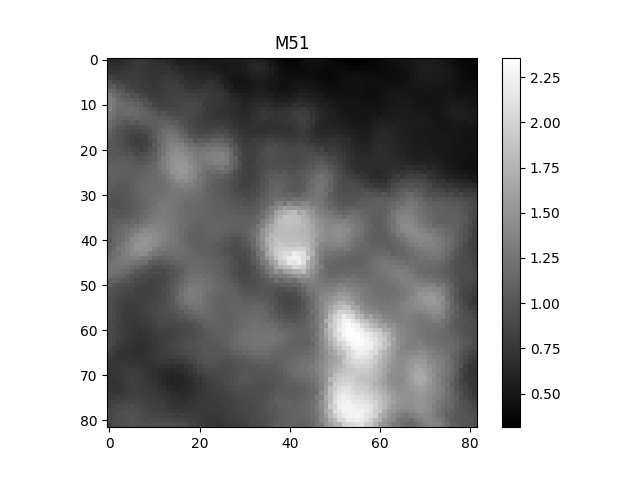
\includegraphics[width=\textwidth]{M51.png}
    \caption{Picture 1}
    \label{fig:1}
  \end{subfigure}
  %
  \begin{subfigure}[b]{0.4\textwidth}
    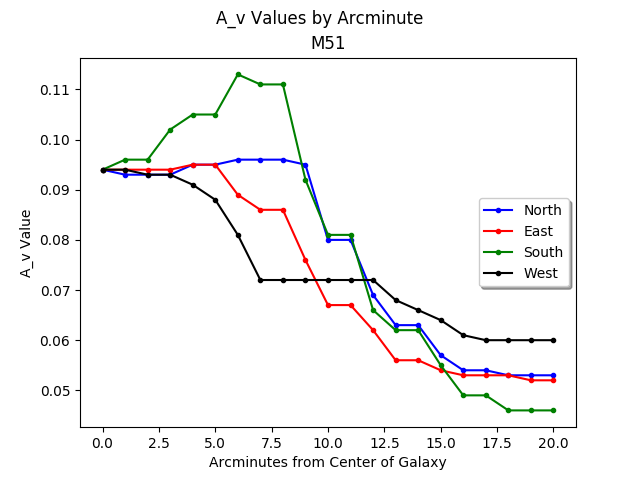
\includegraphics[width=\textwidth]{M51e.png}
    \caption{Picture 2}
    \label{fig:2}
  \end{subfigure}
\end{figure}






\hline
\hline
\end{tabular}
\end{table*}

%%%%%%%%%%%%%%%%
\section{Saving the World, one extinction value at a time  \label{sec_templates}}

Is it better to underestimate, rather than overestimate galactic reddening?

You still have the issue of misascribing how much is from the host.  But if you have to little MW reddening and infer a little more host reddening, that is better than assuming to much and assuming the host has less reddening especially if you get down to no host reddening.  Just increase uncertainties?



%%%%%%%%%%%%%%%%%%%%%%%
\section{Summary\label{sec_summary}}

In summary, we are very concerned about dust reddening.  You should be too.

\acknowledgments



% Facilities 

\vspace{5mm}
%\facilities{HST(STIS), Swift(UVOT)}

\software{
IDL
astropy \citep{2013A&A...558A..33A},  
%          Cloudy \citep{2013RMxAA..49..137F}, 
%          SExtractor \citep{1996A&AS..117..393B}
          }

\bibliographystyle{aasjournal}

\bibliography{bibtex}{}

\end{document}

% End of file